%!TEX TS-program = lualatex
%!TEX encoding = UTF-8 Unicode

\documentclass[12pt]{article}
\usepackage{geometry}
\usepackage{float}
\usepackage{amssymb}
\usepackage{minted}
\usepackage{dirtree}
\usepackage{caption}
\usepackage{adjustbox}
\usepackage[font={small,it}]{caption}
\usepackage{ifxetex,ifluatex}
\usepackage{framed}
\usepackage[12pt]{moresize}
\usepackage{graphicx}
\graphicspath{{./images/}}
\usepackage{booktabs,makecell,multirow,threeparttable}

\usepackage{lscape}
\usepackage{emoji}
\usepackage{array}
\renewcommand{\arraystretch}{1.1}

\usepackage{tikz}
\usetikzlibrary{shapes.multipart}
\usetikzlibrary{positioning}
\usetikzlibrary{shadows}
\usetikzlibrary{calc}
\usepackage{fancyhdr}
\setlength{\headheight}{25pt}
\pagestyle{fancy}
\fancyhf{}
\fancyhead[L]{\leftmark}
\fancyhead[R]{\rightmark}
\fancyfoot[C]{\thepage}
\usepackage{pdflscape}

% \usepackage{fontspec,xltxtra,xunicode,xeCJK}
\usepackage[
  colorlinks=true,
  linkcolor=blue,
  bookmarksnumbered=true,
  CJKbookmarks=true,
  bookmarksopen=true]{hyperref}

\newcommand{\mytitle}[1]{
  {\HUGE \bfseries #1}\par
}

\newcommand{\mysubtitle}[1]{
  {\emph{#1}}\par
}

% \newcommand{\pkfield}[1]{{\color{yellow!60!red}\scalebox{0.6}{\faKey}\ }\texttt{#1}}
% \newcommand{\field}[1]{\phantom{\scalebox{0.6}{\faKey}\ }\texttt{#1}}
\newcommand{\pkfield}[1]{\emoji{key}\ \texttt{#1}}
\newcommand{\field}[1]{\phantom{\emoji{key}\ }\texttt{#1}}
\newcommand{\entity}[1]{\bfseries \texttt{#1}}

\newcommand{\enlargepage}{%
\addtolength{\topmargin}{-2.2cm}
\addtolength{\textheight}{4.4cm}
}

\newcommand{\restorepage}{%
\addtolength{\topmargin}{2.2cm}
\addtolength{\textheight}{-4.4cm}
}

\definecolor{titlepagecolor}{cmyk}{1,.60,0,.40}

\DeclareFixedFont{\titlefont}{T1}{ppl}{b}{it}{1.0in}

\newminted{javascript}{
  autogobble,
  breaklines,
  frame=leftline,
  framerule=1.2pt,
  framesep=1em,
  linenos,
  fontsize=\footnotesize
}

\newminted{sql}{
  autogobble,
  breaklines,
  frame=leftline,
  framerule=1.2pt,
  framesep=1em,
  linenos,
  fontsize=\footnotesize
}

\newminted{bash}{
  autogobble,
  breaklines,
  frame=leftline,
  framerule=1.2pt,
  framesep=1em,
  linenos,
  fontsize=\footnotesize
}

%!TEX TS-program = xelatex
%!TEX r = UTF-8 Unicode
%!TeX root = manual.tex

% conditional for xetex or luatex
\newif\ifxetexorluatex
\ifxetex
  \xetexorluatextrue
\else
  \ifluatex
    \xetexorluatextrue
  \else
    \xetexorluatexfalse
  \fi
\fi
%
\ifxetexorluatex%
  \usepackage{fontspec}
  \usepackage{biolinum}
  \usepackage{libertineRoman} % or use \setmainfont to choose any font on your system
  \newfontfamily\quotefont[Ligatures=TeX]{Linux Libertine O} % selects Libertine as the quote font
\else
  \usepackage[utf8]{inputenc}
  \usepackage[T1]{fontenc}
  \usepackage{biolinum}
  \usepackage{libertineRoman} % or any other font package
  \newcommand*\quotefont{\fontfamily{LinuxLibertineT-LF}} % selects Libertine as the quote font
\fi

\newcommand*\quotesize{60} % if quote size changes, need a way to make shifts relative
% Make commands for the quotes
\newcommand*{\openquote}
   {\tikz[remember picture,overlay,xshift=-4ex,yshift=-2.5ex]
   \node (OQ) {\quotefont\fontsize{\quotesize}{\quotesize}\selectfont``};\kern0pt}

\newcommand*{\closequote}[1]
  {\tikz[remember picture,overlay,xshift=4ex,yshift={#1}]
   \node (CQ) {\quotefont\fontsize{\quotesize}{\quotesize}\selectfont''};}

% select a colour for the shading
\colorlet{shadecolor}{white}

\newcommand*\shadedauthorformat{\emph} % define format for the author argument

% Now a command to allow left, right and centre alignment of the author
\newcommand*\authoralign[1]{%
  \if#1l
    \def\authorfill{}\def\quotefill{\hfill}
  \else
    \if#1r
      \def\authorfill{\hfill}\def\quotefill{}
    \else
      \if#1c
        \gdef\authorfill{\hfill}\def\quotefill{\hfill}
      \else\typeout{Invalid option}
      \fi
    \fi
  \fi}
% wrap everything in its own environment which takes one argument (author) and one optional argument
% specifying the alignment [l, r or c]
%
\newenvironment{shadequote}[2][l]%
{\authoralign{#1}
\ifblank{#2}
   {\def\shadequoteauthor{}\def\yshift{-2ex}\def\quotefill{\hfill}}
   {\def\shadequoteauthor{\par\authorfill\shadedauthorformat{#2}}\def\yshift{2ex}}
\begin{snugshade}\begin{quote}\openquote}
{\shadequoteauthor\quotefill\closequote{\yshift}\end{quote}\end{snugshade}}

%!TEX TS-program = lualatex
%!TEX r = UTF-8 Unicode
%!TeX root = manual.tex

\newcommand\titlepagedecoration{%
\begin{tikzpicture}[remember picture,overlay,shorten >= -10pt]

\coordinate (aux1) at ([yshift=-15pt]current page.north east);
\coordinate (aux2) at ([yshift=-410pt]current page.north east);
\coordinate (aux3) at ([xshift=-4.5cm]current page.north east);
\coordinate (aux4) at ([yshift=-150pt]current page.north east);

\begin{scope}[titlepagecolor!40,line width=12pt,rounded corners=12pt]
\draw
  (aux1) -- coordinate (a)
  ++(225:5) --
  ++(-45:5.1) coordinate (b);
\draw[shorten <= -10pt]
  (aux3) --
  (a) --
  (aux1);
\draw[opacity=0.6,titlepagecolor,shorten <= -10pt]
  (b) --
  ++(225:2.2) --
  ++(-45:2.2);
\end{scope}
\draw[titlepagecolor,line width=8pt,rounded corners=8pt,shorten <= -10pt]
  (aux4) --
  ++(225:0.8) --
  ++(-45:0.8);
\begin{scope}[titlepagecolor!70,line width=6pt,rounded corners=8pt]
\draw[shorten <= -10pt]
  (aux2) --
  ++(225:3) coordinate[pos=0.45] (c) --
  ++(-45:3.1);
\draw
  (aux2) --
  (c) --
  ++(135:2.5) --
  ++(45:2.5) --
  ++(-45:2.5) coordinate[pos=0.3] (d);
\draw
  (d) -- +(45:1);
\end{scope}
\end{tikzpicture}%
}

%!TEX TS-program = lualatex
%!TEX r = UTF-8 Unicode
%!TeX root = manual.tex

% code for "one to omany", etc. is taken from https://tex.stackexchange.com/q/141797/101651
\makeatletter
\pgfarrowsdeclare{crow's foot}{crow's foot}
{
    \pgfarrowsleftextend{+-.5\pgflinewidth}%
    \pgfarrowsrightextend{+.5\pgflinewidth}%
}
{
    \pgfutil@tempdima=0.6pt%
    \pgfsetdash{}{+0pt}%
    \pgfsetmiterjoin%
    \pgfpathmoveto{\pgfqpoint{0pt}{-9\pgfutil@tempdima}}%
    \pgfpathlineto{\pgfqpoint{-13\pgfutil@tempdima}{0pt}}%
    \pgfpathlineto{\pgfqpoint{0pt}{9\pgfutil@tempdima}}%
    \pgfpathmoveto{\pgfqpoint{0\pgfutil@tempdima}{0\pgfutil@tempdima}}%
    \pgfpathmoveto{\pgfqpoint{-8pt}{-6pt}}% 
    \pgfpathlineto{\pgfqpoint{-8pt}{-6pt}}%  
    \pgfpathlineto{\pgfqpoint{-8pt}{6pt}}% 
    \pgfusepathqstroke%
}

\pgfarrowsdeclare{omany}{omany}
{
    \pgfarrowsleftextend{+-.5\pgflinewidth}%
    \pgfarrowsrightextend{+.5\pgflinewidth}%
}
{
    \pgfutil@tempdima=0.6pt%
    \pgfsetdash{}{+0pt}%
    \pgfsetmiterjoin%
    \pgfpathmoveto{\pgfqpoint{0pt}{-9\pgfutil@tempdima}}%
    \pgfpathlineto{\pgfqpoint{-13\pgfutil@tempdima}{0pt}}%
    \pgfpathlineto{\pgfqpoint{0pt}{9\pgfutil@tempdima}}%
    \pgfpathmoveto{\pgfqpoint{0\pgfutil@tempdima}{0\pgfutil@tempdima}}%  
    \pgfpathmoveto{\pgfqpoint{0\pgfutil@tempdima}{0\pgfutil@tempdima}}%
    \pgfpathmoveto{\pgfqpoint{-6pt}{-6pt}}% 
    \pgfpathcircle{\pgfpoint{-11.5pt}{0}} {3.5pt}
    \pgfusepathqstroke%
}

\pgfarrowsdeclare{one}{one}
{
    \pgfarrowsleftextend{+-.5\pgflinewidth}%
    \pgfarrowsrightextend{+.5\pgflinewidth}%
}
{
    \pgfutil@tempdima=0.6pt%
    \pgfsetdash{}{+0pt}%
    \pgfsetmiterjoin%
    \pgfpathmoveto{\pgfqpoint{0\pgfutil@tempdima}{0\pgfutil@tempdima}}%
    \pgfpathmoveto{\pgfqpoint{-6pt}{-6pt}}% 
    \pgfpathlineto{\pgfqpoint{-6pt}{-6pt}}%  
    \pgfpathlineto{\pgfqpoint{-6pt}{6pt}}% 
    \pgfpathmoveto{\pgfqpoint{0\pgfutil@tempdima}{0\pgfutil@tempdima}}%
    \pgfpathmoveto{\pgfqpoint{-8pt}{-6pt}}% 
    \pgfpathlineto{\pgfqpoint{-8pt}{-6pt}}%  
    \pgfpathlineto{\pgfqpoint{-8pt}{6pt}}%    
    \pgfusepathqstroke%
}
\makeatother

\tikzset{%
    pics/entity/.style n args={3}{code={%
        \node[draw,
        rectangle split,
        rectangle split parts=2,
        text height=1.5ex,
        ] (#1)
        {#2 \nodepart{second}
            \begin{tabular}{>{\raggedright\arraybackslash}p{8.5em}}
                #3
            \end{tabular}
        };%
    }},
    pics/entitynoatt/.style n args={2}{code={%
        \node[draw,
        text height=1.5ex,
        ] (#1)
        {#2};%
    }},
    zig zag to/.style={
        to path={(\tikztostart) -| ($(\tikztostart)!#1!(\tikztotarget)$) |- (\tikztotarget)}
    },
    zig zag to/.default=0.5,   
    one to one/.style={
        one-one, zig zag to
    },
    one to oone/.style={            % I do not how to make "one to Optional-one" rel
        one-one, zig zag to
    },
    one to many/.style={
        one-crow's foot, zig zag to,
    },
    one to omany/.style={
        one-omany, zig zag to
    }
}


\begin{document}

\begin{titlepage}
\begin{minipage}{0.8\linewidth}
  \vspace*{4cm}
  \begin{center}
    \noindent
    \mytitle{MongoDB Tutorial}
    \rule{\linewidth}{0.2ex}\par
    \mysubtitle{tutorialpoint.com \\ typeset by Justin Zhang}
  \end{center}
\end{minipage}
\null \vfill
\hfill
\begin{minipage}{0.55\linewidth}
  \begin{flushright}
    % \printauthor
  \end{flushright}
\end{minipage}
%
% \begin{minipage}{0.02\linewidth}
%   \rule{1pt}{260pt}
% \end{minipage}
\titlepagedecoration
\end{titlepage}

\newpage
\tableofcontents
% \newpage
% \listoffigures
% \newpage
% \listoftables
% \newpage
% \listoflistings

\newpage
\thispagestyle{empty}
\topskip0pt
\vspace*{\fill}
This document is typesetted by \href{mailto:schnell18@gmail.com}{\emph{Justin
Zhang}} in \LaTeX\ for better screen reading experience. You
may read the document in its original form at\\
\href{https://www.tutorialspoint.com/mongodb/index.htm}{https://www.tutorialspoint.com/mongodb/index.htm}.
\vspace*{\fill}

\newpage
\thispagestyle{empty}
\topskip0pt
\vspace*{\fill}
\begin{shadequote}[r]{-- Anonymous}
MongoDB is an open-source document database and leading NoSQL database.
MongoDB is written in C++. This tutorial will give you great
understanding on MongoDB concepts needed to create and deploy a highly
\end{shadequote}

\vspace*{\fill}

\newpage
\section{Audience}

This tutorial is designed for Software Professionals who are willing to
learn MongoDB Database in simple and easy steps. It will throw light on
MongoDB concepts and after completing this tutorial you will be at an
intermediate level of expertise, from where you can take yourself at
higher level of expertise.

\newpage
\section{Prerequisites}

Before proceeding with this tutorial, you should have a basic
understanding of database, text editor and execution of programs, etc.
Because we are going to develop high performance database, so it will be
good if you have an understanding on the basic concepts of Database
(RDBMS).

\newpage

\section{Overview}

MongoDB is a cross-platform, document oriented database that provides,
high performance, high availability, and easy scalability. MongoDB works
on concept of collection and document.

\subsection{Database}

Database is a physical container for collections. Each database gets its
own set of files on the file system. A single MongoDB server typically
has multiple databases.

\subsection{Collection}

Collection is a group of MongoDB documents. It is the equivalent of an
RDBMS table. A collection exists within a single database. Collections
do not enforce a schema. Documents within a collection can have
different fields. Typically, all documents in a collection are of
similar or related purpose.

\subsection{Document}

A document is a set of key-value pairs. Documents have dynamic schema.
Dynamic schema means that documents in the same collection do not need
to have the same set of fields or structure, and common fields in a
collection's documents may hold different types of data.

The following table shows the relationship of RDBMS terminology with MongoDB.

\begin{table}[H]
\centering
\begin{threeparttable}
\begin{tabular}{ll}
  \toprule
  \thead{RDBMS} & \thead{MongoDB} \\
  \midrule
  Database & Database \\
  Table & Collection \\
  Tuple/Row & Document \\
  column & Field \\
  Table Join & Embedded Documents \\
  Primary Key & Primary Key (Default key \_id provided by MongoDB itself) \\
  mysqld/Oracle & mongod \\
  mysql/sqlplus & mongo \\
  \bottomrule\addlinespace[1ex]
\end{tabular}
% \begin{tablenotes}
% \end{tablenotes}
\end{threeparttable}
  \caption{MongoDB vs RDBMS}
  \label{tab:mongo-vs-rdbms}
\end{table}


Sample Document

Following example shows the document structure of a blog site, which is
simply a comma separated key value pair.

\begin{javascriptcode}
{
   _id: ObjectId(7df78ad8902c)
   title: 'MongoDB Overview',
   description: 'MongoDB is no sql database',
   by: 'tutorials point',
   url: 'http://www.tutorialspoint.com',
   tags: ['mongodb', 'database', 'NoSQL'],
   likes: 100,
   comments: [
      {
         user:'user1',
         message: 'My first comment',
         dateCreated: new Date(2011,1,20,2,15),
         like: 0
      },
      {
         user:'user2',
         message: 'My second comments',
         dateCreated: new Date(2011,1,25,7,45),
         like: 5
      }
   ]
}
\end{javascriptcode}

\verb=_id= is a 12 bytes hexadecimal number which assures the uniqueness
of every document. You can provide \verb=_id= while inserting the
document. If you don’t provide then MongoDB provides a unique id for
every document. These 12 bytes first 4 bytes for the current timestamp,
next 3 bytes for machine id, next 2 bytes for process id of MongoDB
server and remaining 3 bytes are simple incremental VALUE.

Any relational database has a typical schema design that shows number of
tables and the relationship between these tables. While in MongoDB,
there is no concept of relationship.

\subsection{Advantages of MongoDB over RDBMS}

\begin{itemize}
  \item Schema less -- MongoDB is a document database in which one
    collection holds different documents. Number of fields, content and
    size of the document can differ from one document to another.

  \item Structure of a single object is clear.

  \item No complex joins.

  \item Deep query-ability. MongoDB supports dynamic queries on
    documents using a document-based query language that's nearly as
    powerful as SQL.

  \item Tuning.

  \item Ease of scale-out -− MongoDB is easy to scale.

  \item Conversion/mapping of application objects to database objects not needed.

  \item Uses internal memory for storing the (windowed) working set,
    enabling faster access of data.
\end{itemize}

\subsection{Why Use MongoDB}

\begin{itemize}
  \item Document Oriented Storage − Data is stored in the form of JSON style documents.
  \item Index on any attribute
  \item Replication and high availability
  \item Auto-Sharding
  \item Rich queries
  \item Fast in-place updates
  \item Professional support by MongoDB
\end{itemize}

\subsection{Where to Use MongoDB?}

\begin{itemize}
  \item Big Data
  \item Content Management and Delivery
  \item Mobile and Social Infrastructure
  \item User Data Management
  \item Data Hub
\end{itemize}

\newpage
\section{Data Model}

Data in MongoDB has a flexible schema.documents in the same collection.
They do not need to have the same set of fields or structure Common
fields in a collection’s documents may hold different types of data.

\subsection{Data Model Design}

MongoDB provides two types of data models: — Embedded data model and
Normalized data model. Based on the requirement, you can use either of
the models while preparing your document.

\subsubsection{Embedded Data Model}

In this model, you can have (embed) all the related data in a single
document, it is also known as de-normalized data model.

For example, assume we are getting the details of employees in three
different documents namely, Personal\_details, Contact and, Address, you
can embed all the three documents in a single one as shown below

\begin{javascriptcode}
{
    _id: ,
    Emp_ID: "10025AE336"
    Personal_details:{
        First_Name: "Radhika",
        Last_Name: "Sharma",
        Date_Of_Birth: "1995-09-26"
    },
    Contact: {
        e-mail: "radhika_sharma.123@gmail.com",
        phone: "9848022338"
    },
    Address: {
        city: "Hyderabad",
        Area: "Madapur",
        State: "Telangana"
    }
}
\end{javascriptcode}

\subsubsection{Normalized Data Model}

In this model, you can refer the sub documents in the original document,
using references. For example, you can re-write the above document in
the normalized model as:

Employee:

\begin{javascriptcode}
{
    _id: <ObjectId101>,
    Emp_ID: "10025AE336"
}
\end{javascriptcode}

Personal\_details:

\begin{javascriptcode}
{
    _id: <ObjectId102>,
    empDocID: " ObjectId101",
    First_Name: "Radhika",
    Last_Name: "Sharma",
    Date_Of_Birth: "1995-09-26"
}
\end{javascriptcode}

Contact:

\begin{javascriptcode}
{
    _id: <ObjectId103>,
    empDocID: " ObjectId101",
    e-mail: "radhika_sharma.123@gmail.com",
    phone: "9848022338"
}
\end{javascriptcode}

Address:

\begin{javascriptcode}
{
    _id: <ObjectId104>,
    empDocID: " ObjectId101",
    city: "Hyderabad",
    Area: "Madapur",
    State: "Telangana"
}
\end{javascriptcode}

\subsubsection{Considerations while designing Schema in MongoDB}

\begin{itemize}
  \item Design your schema according to user requirements.

  \item Combine objects into one document if you will use them together.
    Otherwise separate them (but make sure there should not be need of
    joins).

  \item Duplicate the data (but limited) because disk space is cheap as compare to compute time.
  \item Do joins while write, not on read.
  \item Optimize your schema for most frequent use cases.
  \item Do complex aggregation in the schema.
\end{itemize}


\subsection{Example}

Suppose a client needs a database design for his blog/website and see
the differences between RDBMS and MongoDB schema design. Website has the
following requirements.

\begin{itemize}
  \item Every post has the unique title, description and url.
  \item Every post can have one or more tags.
  \item Every post has the name of its publisher and total number of likes.
  \item Every post has comments given by users along with their name,
    message, data-time and likes.
  \item On each post, there can be zero or more comments.
\end{itemize}

In RDBMS schema, design for above requirements will have minimum three
tables as follows:
\begin{figure}[H]
  \begin{tikzpicture}
      \pic {entity={A}{\entity{comments}}{%
        \pkfield{post\_id} \\
        \field{by\_user} \\
        \field{message} \\
        \field{date\_time} \\
        \field{likes}
      }};
      \pic[right=7em of A] {entity={B}{\entity{post}}{%
        \pkfield{id} \\
        \field{title} \\
        \field{description} \\
        \field{url} \\
        \field{likes} \\
        \field{post\_by}
      }};
      \pic[below=7em of B] {entity={C}{\entity{tag\_list}}{%
        \pkfield{id} \\
        \field{post\_id} \\
        \field{tag}
      }};
      \draw[one to omany] (B.west) -- node[above]{\footnotesize has} (A.east);
      \draw[one to omany] (B.south) -- node[above]{\footnotesize has} (C.north);
      \end{tikzpicture}
  \caption{Entity-Relation Diagram}
  \label{fig:er-diagram}
\end{figure}

While in MongoDB schema, design will have one collection post and the following structure −

\begin{javascriptcode}
{
   _id: POST_ID
   title: TITLE_OF_POST,
   description: POST_DESCRIPTION,
   by: POST_BY,
   url: URL_OF_POST,
   tags: [TAG1, TAG2, TAG3],
   likes: TOTAL_LIKES,
   comments: [
      {
         user:'COMMENT_BY',
         message: TEXT,
         dateCreated: DATE_TIME,
         like: LIKES
      },
      {
         user:'COMMENT_BY',
         message: TEXT,
         dateCreated: DATE_TIME,
         like: LIKES
      }
   ]
}
\end{javascriptcode}

So while showing the data, in RDBMS you need to join three tables and in
MongoDB, data will be shown from one collection only.

\newpage
\section{Data Manipulation and Query}
\subsection{Database}

In this chapter, we will see how to create a database in MongoDB.

\subsubsection{Create Database}

MongoDB \emph{use DATABASE} is used to create database. The
command will create a new database if it doesn't exist, otherwise it
will return the existing database.

Basic syntax of use DATABASE statement is as follows:

\begin{bashcode}
use DATABASE
\end{bashcode}

For example, if you want to use a database with name <mydb>, then use
DATABASE statement would be as follows:

\begin{bashcode}
>use mydb
switched to db mydb
\end{bashcode}

To check your currently selected database, use the command db

\begin{bashcode}
>db
mydb
\end{bashcode}

If you want to check your databases list, use the command show dbs.

\begin{bashcode}
>show dbs
local 0.78125GB
test 0.23012GB
\end{bashcode}

Your created database (mydb) is not present in list. To display
database, you need to insert at least one document into it.

\begin{bashcode}
>db.movie.insert({"name":"tutorials point"})
>show dbs
local      0.78125GB
mydb       0.23012GB
test       0.23012GB
\end{bashcode}

In MongoDB default database is test. If you didn't create any database,
then collections will be stored in test database.

\subsubsection{Drop Database}

In this chapter, we will see how to drop a database using MongoDB
command. The MongoDB \emph{db.dropDatabase()} command is used to drop a
existing database. Basic syntax of dropDatabase() command is as follows:

\begin{bashcode}
db.dropDatabase()
\end{bashcode}

This will delete the selected database. If you have not selected any
database, then it will delete default 'test' database.

First, check the list of available databases by using the command, show dbs.

\begin{bashcode}
>show dbs
local      0.78125GB
mydb       0.23012GB
test       0.23012GB
>
\end{bashcode}

If you want to delete new database \emph{mydb}, use
\emph{dropDatabase()} command would be as follows:

\begin{bashcode}
>use mydb
switched to db mydb
>db.dropDatabase()
>{ "dropped" : "mydb", "ok" : 1 }
>
\end{bashcode}

Now check list of databases.

\begin{bashcode}
>show dbs
local      0.78125GB
test       0.23012GB
>
\end{bashcode}

\newpage
\subsection{Collection}
\subsubsection{Create Collection}

In this chapter, we will see how to create a collection using MongoDB.

The MongoDB command \emph{db.createCollection(name, options)} is used to
create collection. Basic syntax of createCollection() command is as
follows:

\begin{bashcode}
db.createCollection(name, options)
\end{bashcode}

In the command, name is name of collection to be created. Options is a
document and is used to specify configuration of collection.
The table \nameref{tab:mongo-create-collection-options} describes
these options.

\begin{table}[H]
\centering
\begin{threeparttable}
  \begin{tabular}{llp{20em}}
  \toprule
  \thead{\bfseries Field} & \thead{\bfseries Type} & \thead{\bfseries Description} \\
  \midrule
    capped & Boolean(Optional) & If true, enables a capped collection. Capped collection is a fixed size collection that automatically overwrites its oldest entries when it reaches its maximum size. If you specify true, you need to specify size parameter also.\\
autoIndexId & Boolean(Optional) & If true, automatically create index on
    \_id field.s Default value is false.\\
size & number(Optional) & Specifies a maximum size in bytes for a capped collection. If capped is true, then you need to specify this field also.\\
max & number(Optional) & Specifies the maximum number of documents allowed in the capped collection.\\
  \bottomrule\addlinespace[1ex]
\end{tabular}
% \begin{tablenotes}
% \end{tablenotes}
\end{threeparttable}
  \caption{Options of db.createCollection() }
  \label{tab:mongo-create-collection-options}
\end{table}

While inserting the document, MongoDB first checks size field of capped
collection, then it checks max field. Basic syntax of method
\emph{createCollection()} without options is as follows:

\begin{bashcode}
>use test
switched to db test
>db.createCollection("mycollection")
{ "ok" : 1 }
>
\end{bashcode}

You can check the created collection by using the command show collections.

\begin{bashcode}
>show collections
mycollection
system.indexes
\end{bashcode}

The following example shows the syntax of createCollection() method with few important options −

\begin{bashcode}
> db.createCollection("mycol", { capped : true, autoIndexID : true, size : 6142800, max : 10000 } ){
"ok" : 0,
"errmsg" : "BSON field 'create.autoIndexID' is an unknown field.",
"code" : 40415,
"codeName" : "Location40415"
}
>
\end{bashcode}

In MongoDB, you don't need to create collection. MongoDB creates
collection automatically, when you insert some document.

\begin{bashcode}
>db.tutorialspoint.insert({"name" : "tutorialspoint"}),
WriteResult({ "nInserted" : 1 })
>show collections
mycol
mycollection
system.indexes
tutorialspoint
>
\end{bashcode}

\subsubsection{Drop Collection}

In this chapter, we will see how to drop a collection using MongoDB.
MongoDB's \emph{db.collection.drop()} method is used to drop a
collection from the database. Basic syntax of drop() command is as
follows:

\begin{bashcode}
db.COLLECTION.drop()
\end{bashcode}

First, check the available collections into your database mydb.

\begin{bashcode}
>use mydb
switched to db mydb
>show collections
mycol
mycollection
system.indexes
tutorialspoint
>
\end{bashcode}

Now drop the collection with the name \emph{mycollection}.

\begin{bashcode}
>db.mycollection.drop()
true
>
\end{bashcode}

Again check the list of collections into database.

\begin{bashcode}
>show collections
mycol
system.indexes
tutorialspoint
>
\end{bashcode}
The \emph{drop()} method will return true, if the selected collection is
dropped successfully, otherwise it will return false.

\subsection{Document}

MongoDB supports many datatypes. Some of them are: \\

  \begin{tabular}{lp{24em}}
    \bfseries String & This is the most commonly used datatype to store the
    data. String in MongoDB must be UTF-8 valid. \\

    \bfseries Integer & This type is used to store a numerical value. Integer
    can be 32 bit or 64 bit depending upon your server. \\

    \bfseries Boolean & This type is used to store a boolean (true/ false) value. \\

    \bfseries Double & This type is used to store floating point values. \\

    \bfseries Min/ Max keys & This type is used to compare a value against the
    lowest and highest BSON elements. \\

    \bfseries Arrays & This type is used to store arrays or list or multiple
    values into one key. \\

    \bfseries Timestamp & ctimestamp. This can be handy for recording when a
    document has been modified or added. \\

    \bfseries Object & This datatype is used for embedded documents. \\

    \bfseries Null & This type is used to store a Null value. \\

    \bfseries Symbol & This datatype is used identically to a string; however,
    it's generally reserved for languages that use a specific symbol
    type. \\

    \bfseries Date & This datatype is used to store the current date or time in
    UNIX time format. You can specify your own date time by creating
    object of Date and passing day, month, year into it. \\

    \bfseries Object ID & This datatype is used to store the document’s ID. \\
    \bfseries Binary data & This datatype is used to store binary data. \\
    \bfseries Code & This datatype is used to store JavaScript code into the document. \\
    \bfseries Regular expression & This datatype is used to store regular expression. \\
\end{tabular}

\subsubsection{Insert Document}

In this chapter, we will learn how to insert document in MongoDB collection.

To insert data into MongoDB collection, you need to use MongoDB's
\emph{insert()} or \emph{save()} method. The basic syntax of insert()
command is as follows:

\begin{bashcode}
>db.COLLECTION.insert(document)
Example
> db.users.insert({
... _id : ObjectId("507f191e810c19729de860ea"),
... title: "MongoDB Overview",
... description: "MongoDB is no sql database",
... by: "tutorials point",
... url: "http://www.tutorialspoint.com",
... tags: ['mongodb', 'database', 'NoSQL'],
... likes: 100
... })
WriteResult({ "nInserted" : 1 })
>
\end{bashcode}

Here \emph{mycol} is our collection name, as created in the previous
chapter. If the collection doesn't exist in the database, then MongoDB
will create this collection and then insert a document into it.

In the inserted document, if we don't specify the \_id parameter, then
MongoDB assigns a unique ObjectId for this document.

\_id is 12 bytes hexadecimal number unique for every document in a
collection. 12 bytes are divided as follows:

\begin{enumerate}
  \item 4 bytes timestamp
  \item 3 bytes machine id
  \item 2 bytes process id
  \item 3 bytes incrementer
\end{enumerate}

You can also pass an array of documents into the insert() method as
shown below:

\begin{bashcode}
> db.createCollection("post")
> db.post.insert([
    {
        title: "MongoDB Overview",
        description: "MongoDB is no SQL database",
        by: "tutorials point",
        url: "http://www.tutorialspoint.com",
        tags: ["mongodb", "database", "NoSQL"],
        likes: 100
    },
    {
    title: "NoSQL Database",
    description: "NoSQL database doesn't have tables",
    by: "tutorials point",
    url: "http://www.tutorialspoint.com",
    tags: ["mongodb", "database", "NoSQL"],
    likes: 20,
    comments: [
        {
            user:"user1",
            message: "My first comment",
            dateCreated: new Date(2013,11,10,2,35),
            like: 0
        }
    ]
}
])
BulkWriteResult({
    "writeErrors" : [ ],
    "writeConcernErrors" : [ ],
    "nInserted" : 2,
    "nUpserted" : 0,
    "nMatched" : 0,
    "nModified" : 0,
    "nRemoved" : 0,
    "upserted" : [ ]
})
>
\end{bashcode}

To insert the document you can also use the
\emph{db.post.save(document)} method. If you don't specify \_id in the
document then save() method will work same as \emph{insert()} method. If
you specify \_id then it will replace whole data of document containing
\_id as specified in \emph{save()} method.

If you need to insert only one document into a collection you can use
the method \emph{insertOne()}.
The basic syntax of this method is as follows:

\begin{bashcode}
>db.COLLECTION_NAME.insertOne(document)
\end{bashcode}

Following example creates a new collection named \emph{empDetails} and
inserts a document using the \emph{insertOne()} method.

\begin{bashcode}
> db.createCollection("empDetails")
{ "ok" : 1 }
> db.empDetails.insertOne(
    {
        First_Name: "Radhika",
        Last_Name: "Sharma",
        Date_Of_Birth: "1995-09-26",
        e_mail: "radhika_sharma.123@gmail.com",
        phone: "9848022338"
    })
{
    "acknowledged" : true,
    "insertedId" : ObjectId("5dd62b4070fb13eec3963bea")
}
>
\end{bashcode}

You can insert multiple documents using the \emph{insertMany()} method.
To use this method you need to pass an array of documents. Following
example inserts three different documents into the \emph{empDetails} collection
using the \emph{insertMany()} method.

\begin{bashcode}
> db.empDetails.insertMany(
    [
        {
            First_Name: "Radhika",
            Last_Name: "Sharma",
            Date_Of_Birth: "1995-09-26",
            e_mail: "radhika_sharma.123@gmail.com",
            phone: "9000012345"
        },
        {
            First_Name: "Rachel",
            Last_Name: "Christopher",
            Date_Of_Birth: "1990-02-16",
            e_mail: "Rachel_Christopher.123@gmail.com",
            phone: "9000054321"
        },
        {
            First_Name: "Fathima",
            Last_Name: "Sheik",
            Date_Of_Birth: "1990-02-16",
            e_mail: "Fathima_Sheik.123@gmail.com",
            phone: "9000054321"
        }
    ]
)
{
    "acknowledged" : true,
    "insertedIds" : [
        ObjectId("5dd631f270fb13eec3963bed"),
        ObjectId("5dd631f270fb13eec3963bee"),
        ObjectId("5dd631f270fb13eec3963bef")
    ]
}
>
\end{bashcode}

\newpage
\subsubsection{Query Document}

In this chapter, we will learn how to query document from MongoDB collection.
To query data from MongoDB collection, you need to use MongoDB's
\emph{find()} method. The basic syntax of find() method is as follows:

\begin{bashcode}
>db.COLLECTION.find()
\end{bashcode}

The \emph{find()} method will display all the documents in a non-structured way.

Assume we have created a collection named \emph{mycol} as follows:

\begin{bashcode}
> use sampleDB
switched to db sampleDB
> db.createCollection("mycol")
{ "ok" : 1 }
>
\end{bashcode}

And inserted 3 documents in it using the \emph{insert()} method as shown
below:

\begin{bashcode}
> db.mycol.insert([
    {
        title: "MongoDB Overview",
        description: "MongoDB is no SQL database",
        by: "tutorials point",
        url: "http://www.tutorialspoint.com",
        tags: ["mongodb", "database", "NoSQL"],
        likes: 100
    },
    {
        title: "NoSQL Database",
        description: "NoSQL database doesn't have tables",
        by: "tutorials point",
        url: "http://www.tutorialspoint.com",
        tags: ["mongodb", "database", "NoSQL"],
        likes: 20,
        comments: [
            {
                user:"user1",
                message: "My first comment",
                dateCreated: new Date(2013,11,10,2,35),
                like: 0
            }
        ]
    }
])
\end{bashcode}

Following method retrieves all the documents in the collection:

\begin{bashcode}
> db.mycol.find()
{ "_id" : ObjectId("5dd4e2cc0821d3b44607534c"), "title" : "MongoDB Overview", "description" : "MongoDB is no SQL database", "by" : "tutorials point", "url" : "http://www.tutorialspoint.com", "tags" : [ "mongodb", "database", "NoSQL" ], "likes" : 100 }
{ "_id" : ObjectId("5dd4e2cc0821d3b44607534d"), "title" : "NoSQL Database", "description" : "NoSQL database doesn't have tables", "by" : "tutorials point", "url" : "http://www.tutorialspoint.com", "tags" : [ "mongodb", "database", "NoSQL" ], "likes" : 20, "comments" : [ { "user" : "user1", "message" : "My first comment", "dateCreated" : ISODate("2013-12-09T21:05:00Z"), "like" : 0 } ] }
>
\end{bashcode}

To display the results in a formatted way, you can use the
\emph{pretty()} method. Following example retrieves all the documents
from the collection named \emph{mycol} and arranges them in an
easy-to-read format.

\begin{bashcode}
> db.mycol.find().pretty()
{
    "_id" : ObjectId("5dd4e2cc0821d3b44607534c"),
    "title" : "MongoDB Overview",
    "description" : "MongoDB is no SQL database",
    "by" : "tutorials point",
    "url" : "http://www.tutorialspoint.com",
    "tags" : [
        "mongodb",
        "database",
        "NoSQL"
    ],
    "likes" : 100
}
{
    "_id" : ObjectId("5dd4e2cc0821d3b44607534d"),
    "title" : "NoSQL Database",
    "description" : "NoSQL database doesn't have tables",
    "by" : "tutorials point",
    "url" : "http://www.tutorialspoint.com",
    "tags" : [
        "mongodb",
        "database",
        "NoSQL"
    ],
    "likes" : 20,
    "comments" : [
        {
            "user" : "user1",
            "message" : "My first comment",
            "dateCreated" : ISODate("2013-12-09T21:05:00Z"),
            "like" : 0
        }
    ]
}
\end{bashcode}

Apart from the \emph{find()} method, there is \emph{findOne()} method,
which returns only one document.

Following example retrieves the document with title MongoDB Overview.

\begin{bashcode}
> db.mycol.findOne({title: "MongoDB Overview"})
{
    "_id" : ObjectId("5dd6542170fb13eec3963bf0"),
    "title" : "MongoDB Overview",
    "description" : "MongoDB is no SQL database",
    "by" : "tutorials point",
    "url" : "http://www.tutorialspoint.com",
    "tags" : [
        "mongodb",
        "database",
        "NoSQL"
    ],
    "likes" : 100
}
\end{bashcode}

To query the document on the basis of some condition, you can use following operations.


\begin{table}[H]
\centering
\begin{threeparttable}
  \begin{tabular}{lp{10em}p{12em}p{8em}}
  \toprule
  \thead{\bfseries Op} & \thead{\bfseries Syntax} &
  \thead{\bfseries Example} & \thead{\bfseries RDBMS Equivalent} \\
  \midrule
=  & \{<key>:\{\$eg;<value>\}\} & db.mycol.find(\{"by":"tutorials point"\}) &  where by = 'tutorials point' \\
<  &  \{<key>:\{\$lt:<value>\}\} & db.mycol.find(\{"likes":\{\$lt:50\}\}) & where likes < 50 \\
<= &   \{<key>:\{\$lte:<value>\}\} & db.mycol.find(\{"likes":\{\$lte:50\}\}) & where likes <= 50 \\
>  &   \{<key>:\{\$gt:<value>\}\} & db.mycol.find(\{"likes":\{\$gt:50\}\}) & where likes > 50 \\
>= & \{<key>:\{\$gte:<value>\}\} & db.mycol.find(\{"likes":\{\$gte:50\}\}) &where likes >= 50 \\
!= & \{<key>:\{\$ne:<value>\}\} & db.mycol.find(\{"likes":\{\$ne:50\}\})  &where likes != 50 \\
in &  \{<key>:\{\$in:[<value1>, <value2>,……<valueN>]\}\} & db.mycol.find(\{"name":\{\$in:["ac", "ef", "jc"]\}\}) & where name in ('ac', 'ef', 'jc') \\
not in & \{<key>:\{\$nin:<value>\}\} & db.mycol.find(\{"name":\{\$nin:["ac", "xy"]\}\})  & where name not in ('ac', 'xy') \\
  \bottomrule\addlinespace[1ex]
\end{tabular}
% \begin{tablenotes}
% \end{tablenotes}
\end{threeparttable}
  \caption{RDBMS Where Clause Equivalents in MongoDB}
  \label{tab:mongo-query-criteria}
\end{table}





To query documents based on the AND condition, you need to use \$and
keyword. Following is the basic syntax of AND:

\begin{bashcode}
>db.mycol.find({ $and: [ {<key1>:<value1>}, { <key2>:<value2>} ] })
\end{bashcode}

Following example will show all the tutorials written by 'tutorials
point' and whose title is 'MongoDB Overview'.

\begin{bashcode}
> db.mycol.find({$and:[{"by":"tutorials point"},{"title": "MongoDB Overview"}]}).pretty()
{
    "_id" : ObjectId("5dd4e2cc0821d3b44607534c"),
    "title" : "MongoDB Overview",
    "description" : "MongoDB is no SQL database",
    "by" : "tutorials point",
    "url" : "http://www.tutorialspoint.com",
    "tags" : [
        "mongodb",
        "database",
        "NoSQL"
    ],
    "likes" : 100
}
>
\end{bashcode}

For the above given example, equivalent where clause will be \emph{where by
= 'tutorials point' AND title = 'MongoDB Overview'}. You can pass any
number of key, value pairs in find clause.

To query documents based on the OR condition, you need to use \$or
keyword. Following is the basic syntax of OR:

\begin{bashcode}
>db.mycol.find(
{
$or: [
{key1: value1}, {key2:value2}
]
}
).pretty()
\end{bashcode}

Following example will show all the tutorials written by 'tutorials
point' or whose title is 'MongoDB Overview'.

\begin{bashcode}
>db.mycol.find({$or:[{"by":"tutorials point"},{"title": "MongoDB Overview"}]}).pretty()
{
   "_id": ObjectId(7df78ad8902c),
   "title": "MongoDB Overview", 
   "description": "MongoDB is no sql database",
   "by": "tutorials point",
   "url": "http://www.tutorialspoint.com",
   "tags": ["mongodb", "database", "NoSQL"],
   "likes": "100"
}
>
\end{bashcode}

You may use AND and OR together. The following example will show the
documents that have likes greater than 10 and whose title is either
'MongoDB Overview' or by is 'tutorials point'. Equivalent SQL where
clause is \emph{'where likes>10 AND (by = 'tutorials point' OR title =
'MongoDB Overview')'}

\begin{bashcode}
>db.mycol.find({"likes": {$gt:10}, $or: [{"by": "tutorials point"},
   {"title": "MongoDB Overview"}]}).pretty()
{
   "_id": ObjectId(7df78ad8902c),
   "title": "MongoDB Overview", 
   "description": "MongoDB is no sql database",
   "by": "tutorials point",
   "url": "http://www.tutorialspoint.com",
   "tags": ["mongodb", "database", "NoSQL"],
   "likes": "100"
}
>
\end{bashcode}

To query documents based on the NOT condition, you need to use \$not
keyword. Following is the basic syntax of NOT:

\begin{bashcode}
>db.COLLECTION_NAME.find({$not: [
    {key1: value1}, {key2:value2}
]})
\end{bashcode}

Assume we have inserted 3 documents in the collection empDetails as
shown below:

\begin{bashcode}
db.empDetails.insertMany(
    [
        {
            First_Name: "Radhika",
            Last_Name: "Sharma",
            Age: "26",
            e_mail: "radhika_sharma.123@gmail.com",
            phone: "9000012345"
        },
        {
            First_Name: "Rachel",
            Last_Name: "Christopher",
            Age: "27",
            e_mail: "Rachel_Christopher.123@gmail.com",
            phone: "9000054321"
        },
        {
            First_Name: "Fathima",
            Last_Name: "Sheik",
            Age: "24",
            e_mail: "Fathima_Sheik.123@gmail.com",
            phone: "9000054321"
        }
    ]
)
\end{bashcode}

Following example will retrieve the document(s) whose first name is not
"Radhika" and last name is not "Christopher"

\begin{bashcode}
> db.empDetails.find(
    {
        $nor:[
            40
            {"First_Name": "Radhika"},
            {"Last_Name": "Christopher"}
        ]
    }
).pretty()
{
    "_id" : ObjectId("5dd631f270fb13eec3963bef"),
    "First_Name" : "Fathima",
    "Last_Name" : "Sheik",
    "Age" : "24",
    "e_mail" : "Fathima_Sheik.123@gmail.com",
    "phone" : "9000054321"
}
\end{bashcode}

To query documents based on the NOT condition, you need to use \$not
keyword following is the basic syntax of NOT:

\begin{bashcode}
>db.COLLECTION.find(
{
$NOT: [
{key1: value1}, {key2:value2}
]
}
).pretty()
\end{bashcode}

Following example will retrieve the document(s) whose age is not greater
than 25:

\begin{bashcode}
> db.empDetails.find( { "Age": { $not: { $gt: "25" } } } )
{
    "_id" : ObjectId("5dd6636870fb13eec3963bf7"),
    "First_Name" : "Fathima",
    "Last_Name" : "Sheik",
    "Age" : "24",
    "e_mail" : "Fathima_Sheik.123@gmail.com",
    "phone" : "9000054321"
}
\end{bashcode}

\subsubsection{Update Document}

MongoDB's \emph{update()} and \emph{save()} methods are used to update
document into a collection. The \emph{update()} method updates the
values in the existing document while the \emph{save()} method replaces
the existing document with the document passed in \emph{save()} method.

The basic syntax of \emph{update()} method is as follows:

\begin{bashcode}
>db.COLLECTION_NAME.update(SELECTION_CRITERIA, UPDATED_DATA)
\end{bashcode}
Consider the mycol collection has the following data.

\begin{javascriptcode}
{ "_id" : ObjectId(5983548781331adf45ec5), "title":"MongoDB Overview"}
{ "_id" : ObjectId(5983548781331adf45ec6), "title":"NoSQL Overview"}
{ "_id" : ObjectId(5983548781331adf45ec7), "title":"Tutorials Point Overview"}
\end{javascriptcode}

Following example will set the new title 'New MongoDB Tutorial' of the
documents whose title is 'MongoDB Overview'.

\begin{bashcode}
>db.mycol.update({'title':'MongoDB Overview'},{$set:{'title':'New MongoDB Tutorial'}})
WriteResult({ "nMatched" : 1, "nUpserted" : 0, "nModified" : 1 })
>db.mycol.find()
{ "_id" : ObjectId(5983548781331adf45ec5), "title":"New MongoDB Tutorial"}
{ "_id" : ObjectId(5983548781331adf45ec6), "title":"NoSQL Overview"}
{ "_id" : ObjectId(5983548781331adf45ec7), "title":"Tutorials Point Overview"}
>
\end{bashcode}

By default, MongoDB will update only a single document. To update
multiple documents, you need to set a parameter 'multi' to true.

\begin{bashcode}
>db.mycol.update({'title':'MongoDB Overview'},
   {$set:{'title':'New MongoDB Tutorial'}},{multi:true})
MongoDB Save() Method
The save() method replaces the existing document with the new document passed in the save() method.
\end{bashcode}

The basic syntax of MongoDB save() method is shown below:

\begin{bashcode}
>db.COLLECTION_NAME.save({_id:ObjectId(),NEW_DATA})
\end{bashcode}
Following example will replace the document with the \_id
\emph{'5983548781331adf45ec5'}.

\begin{bashcode}
>db.mycol.save(
   {
      "_id" : ObjectId("507f191e810c19729de860ea"), 
        "title":"Tutorials Point New Topic",
      "by":"Tutorials Point"
   }
)
WriteResult({
    "nMatched" : 0,
    "nUpserted" : 1,
    "nModified" : 0,
    "_id" : ObjectId("507f191e810c19729de860ea")
})
>db.mycol.find()
{ "_id" : ObjectId("507f191e810c19729de860e6"), "title":"Tutorials Point New Topic",
   "by":"Tutorials Point"}
{ "_id" : ObjectId("507f191e810c19729de860e6"), "title":"NoSQL Overview"}
{ "_id" : ObjectId("507f191e810c19729de860e6"), "title":"Tutorials Point Overview"}
>
\end{bashcode}

The \emph{findOneAndUpdate()} method updates the values in the existing
document. The basic syntax of findOneAndUpdate() method is as follows:

\begin{bashcode}
>db.COLLECTION.findOneAndUpdate(SELECTIOIN_CRITERIA, UPDATED_DATA)
\end{bashcode}

Assume we have created a collection named empDetails and inserted three
documents in it as shown below:

\begin{bashcode}
> db.empDetails.insertMany(
    [
        {
            First_Name: "Radhika",
            Last_Name: "Sharma",
            Age: "26",
            e_mail: "radhika_sharma.123@gmail.com",
            phone: "9000012345"
        },
        {
            First_Name: "Rachel",
            Last_Name: "Christopher",
            Age: "27",
            e_mail: "Rachel_Christopher.123@gmail.com",
            phone: "9000054321"
        },
        {
            First_Name: "Fathima",
            Last_Name: "Sheik",
            Age: "24",
            e_mail: "Fathima_Sheik.123@gmail.com",
            phone: "9000054321"
        }
    ]
)
\end{bashcode}

Following example updates the age and email values of the document with
name 'Radhika'.

\begin{bashcode}
> db.empDetails.findOneAndUpdate(
    {First_Name: 'Radhika'},
    { $set: { Age: '30',e_mail: 'radhika_newemail@gmail.com'}}
)
{
    "_id" : ObjectId("5dd6636870fb13eec3963bf5"),
    "First_Name" : "Radhika",
    "Last_Name" : "Sharma",
    "Age" : "30",
    "e_mail" : "radhika_newemail@gmail.com",
    "phone" : "9000012345"
}
\end{bashcode}

The \emph{updateOne()} method updates a single document which matches
the given filter. The basic syntax of updateOne() method is as follows:

\begin{bashcode}
>db.COLLECTION_NAME.updateOne(<filter>, <update>)
\end{bashcode}

The code that follows demonstrates the use of this method:
\begin{bashcode}
> db.empDetails.updateOne(
    {First_Name: 'Radhika'},
    { $set: { Age: '30',e_mail: 'radhika_newemail@gmail.com'}}
)
{ "acknowledged" : true, "matchedCount" : 1, "modifiedCount" : 0 }
>
\begin{bashcode}

The \emph{updateMany()} method updates all the documents that matches
  the given filter. The typical usage of this method is as follows:

\begin{bashcode}
> db.empDetails.updateMany(
    {Age:{ $gt: "25" }},
    { $set: { Age: '00'}}
)
{ "acknowledged" : true, "matchedCount" : 2, "modifiedCount" : 2 }
\end{bashcode}

You can see the updated values if you retrieve the contents of the
  document using the find method as shown below:

\begin{bashcode}
> db.empDetails.find()
{ "_id" : ObjectId("5dd6636870fb13eec3963bf5"), "First_Name" : "Radhika", "Last_Name" : "Sharma", "Age" : "00", "e_mail" : "radhika_newemail@gmail.com", "phone" : "9000012345" }
{ "_id" : ObjectId("5dd6636870fb13eec3963bf6"), "First_Name" : "Rachel", "Last_Name" : "Christopher", "Age" : "00", "e_mail" : "Rachel_Christopher.123@gmail.com", "phone" : "9000054321" }
{ "_id" : ObjectId("5dd6636870fb13eec3963bf7"), "First_Name" : "Fathima", "Last_Name" : "Sheik", "Age" : "24", "e_mail" : "Fathima_Sheik.123@gmail.com", "phone" : "9000054321" }
>
\end{bashcode}

\subsubsection{Delete Document}

In this chapter, we will learn how to delete a document using MongoDB.
  MongoDB's \emph{remove()} method is used to remove a document from the
  collection. This method accepts two parameters. One is deletion
  criteria and second is \emph{justOne} flag. Deletion criteria
  specifies the criteria of documents to be removed. If \emph{justOne}
  is set to true or 1, then this method only remote one document.

  Suppose the \emph{mycol} collection has the following data.

\begin{javascriptcode}
{_id : ObjectId("507f191e810c19729de860e1"), title: "MongoDB Overview"},
{_id : ObjectId("507f191e810c19729de860e2"), title: "NoSQL Overview"},
{_id : ObjectId("507f191e810c19729de860e3"), title: "Tutorials Point Overview"}
\end{javascriptcode}

Following example will remove all the documents whose title is 'MongoDB Overview'.

  \begin{bashcode}
>db.mycol.remove({'title':'MongoDB Overview'})
WriteResult({"nRemoved" : 1})
> db.mycol.find()
{"_id" : ObjectId("507f191e810c19729de860e2"), "title" : "NoSQL Overview" }
{"_id" : ObjectId("507f191e810c19729de860e3"), "title" : "Tutorials Point Overview" }
  \end{bashcode}

If there are multiple records and you want to delete only the first
  record, then set \emph{justOne} parameter in \emph{remove()} method.

  \begin{bashcode}
>db.COLLECTION_NAME.remove(DELETION_CRITERIA,1)
  \end{bashcode}

If you don't specify deletion criteria, then MongoDB will delete whole
  documents from the collection. This is equivalent of SQL's truncate
  command:
\begin{bashcode}
> db.mycol.remove({})
WriteResult({ "nRemoved" : 2 })
> db.mycol.find()
>
\end{bashcode}

\subsubsection{Projection}
In MongoDB, projection means selecting only the necessary data rather
than selecting whole of the data of a document. If a document has 5
fields and you need to show only 3, then select only 3 fields from them.

MongoDB's \emph{find()} method accepts second optional parameter that is
list of fields that you want to retrieve. In MongoDB, when you execute
\emph{find()} method, then it displays all fields of a document. To
limit this, you need to set a list of fields with value 1 or 0. 1 is
used to show the field while 0 is used to hide the fields.

Suppose the collection \emph{mycol} has the following data:

\begin{javascriptcode}
{_id : ObjectId("507f191e810c19729de860e1"), title: "MongoDB Overview"},
{_id : ObjectId("507f191e810c19729de860e2"), title: "NoSQL Overview"},
{_id : ObjectId("507f191e810c19729de860e3"), title: "Tutorials Point Overview"}
\end{javascriptcode}

Following example displays the title of the document:

\begin{bashcode}
>db.mycol.find({},{"title":1,_id:0})
{"title":"MongoDB Overview"}
{"title":"NoSQL Overview"}
{"title":"Tutorials Point Overview"}
>
\end{bashcode}

\subsubsection{Limiting Records}
To limit the records in MongoDB, you need to use \emph{limit()} method. The
method accepts one number type argument, which is the number of
documents that you want to be displayed.

Support the collection \emph{myycol} has the following data:

\begin{javascriptcode}
{_id : ObjectId("507f191e810c19729de860e1"), title: "MongoDB Overview"},
{_id : ObjectId("507f191e810c19729de860e2"), title: "NoSQL Overview"},
{_id : ObjectId("507f191e810c19729de860e3"), title: "Tutorials Point Overview"}
\end{javascriptcode}

Following example displays only two documents:

\begin{bashcode}
>db.mycol.find({},{"title":1,_id:0}).limit(2)
{"title":"MongoDB Overview"}
{"title":"NoSQL Overview"}
>
\end{bashcode}

If you don't specify the number argument in \emph{limit()} method then it will
display all documents from the collection.

Apart from \emph{limit()} method, there is one more method \emph{skip()}
which also accepts number type argument and is used to skip the number
of documents.

Using the previous example of collection \emph{mycol},
the example below displays only the second document.

\begin{bashcode}
>db.mycol.find({},{"title":1,_id:0}).limit(1).skip(1)
{"title":"NoSQL Overview"}
>
\end{bashcode}
The default value of skip() method is 0.

\subsubsection{Sorting Records}

To sort documents in MongoDB, you need to use \emph{sort()} method. The
method accepts a document containing a list of fields along with their
sorting order. To specify sorting order 1 and -1 are used. 1 is used for
ascending order while -1 is used for descending order.

Suppose we have collection \emph{mycol} with the following data:
\begin{javascriptcode}
{_id : ObjectId("507f191e810c19729de860e1"), title: "MongoDB Overview"}
{_id : ObjectId("507f191e810c19729de860e2"), title: "NoSQL Overview"}
{_id : ObjectId("507f191e810c19729de860e3"), title: "Tutorials Point Overview"}
\end{javascriptcode}

Following example displays documents sorted by title in the descending order.

\begin{bashcode}
>db.mycol.find({},{"title":1,_id:0}).sort({"title":-1})
{"title":"Tutorials Point Overview"}
{"title":"NoSQL Overview"}
{"title":"MongoDB Overview"}
>
\end{bashcode}

Please be advised, if you don't specify the sorting preference, then the
\emph{sort()} method will display the documents in ascending order.

\newpage
\subsubsection{Indexing}

Indexes enable efficient resolution of queries. Without indexes, MongoDB
must scan every document of a collection to identify those documents
that match the query statement. The scan is highly inefficient and
requires MongoDB to process a large volume of data. Indexes are special
data structures, that store a small portion of the data set in an
easy-to-traverse form. The index stores the value of a specific field or
set of fields, ordered by the value of the field as specified in the
index.

To create an index, you use the \emph{createIndex()} method.
The basic syntax of this method is as follows:

\begin{bashcode}
>db.COLLECTION.createIndex({KEY:1})
\end{bashcode}

Here key is the name of the field on which you want to create index and
1 is for ascending order. To create index in descending order you need
to use -1.

Here is a concrete example of creating index using the
\emph{createIndex} method:

\begin{bashcode}
>db.mycol.createIndex({"title":1})
{
    "createdCollectionAutomatically" : false,
    "numIndexesBefore" : 1,
    "numIndexesAfter" : 2,
    "ok" : 1
}
>
\end{bashcode}

You can pass multiple fields in \emph{createIndex()} method to create
multi-field index:

\begin{bashcode}
>db.mycol.createIndex({"title":1,"description":-1})
>
\end{bashcode}
This method also accepts list of options (which are optional) as
described in table \nameref{tab:create-index-options}:

\begin{table}[H]
\centering
\begin{threeparttable}
  \begin{tabular}{llp{22em}}
  \toprule
  \thead{\bfseries Parameter} & \thead{\bfseries Type} & \thead{\bfseries Description} \\
  \midrule
background  & Boolean & Builds the index in the background so that building an index does not block other database activities. Specify true to build in the background. The default value is false. \\
unique &  Boolean & Creates a unique index so that the collection will not accept insertion of documents where the index key or keys match an existing value in the index. Specify true to create a unique index. The default value is false. \\
name &    string &  The name of the index. If unspecified, MongoDB generates an index name by concatenating the names of the indexed fields and the sort order. \\
sparse &  Boolean & If true, the index only references documents with the specified field. These indexes use less space but behave differently in some situations (particularly sorts). The default value is false. \\
expireAfterSeconds &  integer & Specifies a value, in seconds, as a TTL to control how long MongoDB retains documents in this collection. \\
weights & document    & The weight is a number ranging from 1 to 99,999 and denotes the significance of the field relative to the other indexed fields in terms of the score. \\
default\_language  & string &For a text index, the language that determines the list of stop words and the rules for the stemmer and tokenizer. The default value is English.\\
language\_override & string &For a text index, specify the name of the field in the document that contains, the language to override the default language. The default value is language. \\
  \bottomrule\addlinespace[1ex]
\end{tabular}
% \begin{tablenotes}
% \end{tablenotes}
\end{threeparttable}
  \caption{Options of createIndex()}
  \label{tab:create-index-options}
\end{table}


You can drop a particular index using the \emph{dropIndex()} method of
MongoDB. The basic syntax of \emph{dropIndex()} method is as follows:
\begin{bashcode}
>db.COLLECTION.dropIndex({KEY:1})
\end{bashcode}
Here, "key" is the name of the file on which you want to remove an
existing index. Instead of the index specification document (above
syntax), you can also specify the name of the index directly as:

\begin{bashcode}
dropIndex("name_of_the_index")
Example
> db.mycol.dropIndex({"title":1})
{
    "ok" : 0,
    "errmsg" : "can't find index with key: { title: 1.0 }",
    "code" : 27,
    "codeName" : "IndexNotFound"
}
\end{bashcode}

The \emph{dropIndexes()} method deletes multiple (specified) indexes on a collection.
The basic syntax of \emph{dropIndexes()} method is as follows:

\begin{bashcode}
>db.COLLECTION.dropIndexes()
\end{bashcode}
Assume we have created 2 indexes in the named mycol collection as shown
below:
\begin{bashcode}
> db.mycol.createIndex({"title":1,"description":-1})
\end{bashcode}
We can drop the indexes as follows:

\begin{bashcode}
>db.mycol.dropIndexes({"title":1,"description":-1})
{ "nIndexesWas" : 2, "ok" : 1 }
>
\end{bashcode}

The \emph{getIndexes()} method returns the description of all the
indexes int the collection. Assume we have created 2 indexes in the
named mycol collection as shown below:

\begin{bashcode}
> db.mycol.createIndex({"title":1,"description":-1})
\end{bashcode}

Following example retrieves all the indexes in the collection
\emph{mycol}:

\begin{bashcode}
> db.mycol.getIndexes()
[
    {
        "v" : 2,
        "key" : {
            "_id" : 1
        },
        "name" : "_id_",
        "ns" : "test.mycol"
    },
    {
        "v" : 2,
        "key" : {
            "title" : 1,
            "description" : -1
        },
        "name" : "title_1_description_-1",
        "ns" : "test.mycol"
    }
]
>
\end{bashcode}

\newpage
\subsubsection{Aggregation}

Aggregation operations process data documents and return computed
results. They group values from multiple documents
together, and perform a variety of operations on the grouped data to
return a single result. You can think of MongoDB's aggregation
operations as something like select count(*) from group by in SQL.
To use aggregation in MongoDB, follow syntax as follows:

\begin{bashcode}
>db.COLLECTION.aggregate(AGGREGATE_OPERATION)
\end{bashcode}

Suppose you have the following data:

\begin{javascriptcode}

{
   _id: ObjectId(7df78ad8902c)
   title: 'MongoDB Overview', 
   description: 'MongoDB is no sql database',
   by_user: 'tutorials point',
   url: 'http://www.tutorialspoint.com',
   tags: ['mongodb', 'database', 'NoSQL'],
   likes: 100
},
{
   _id: ObjectId(7df78ad8902d)
   title: 'NoSQL Overview', 
   description: 'No sql database is very fast',
   by_user: 'tutorials point',
   url: 'http://www.tutorialspoint.com',
   tags: ['mongodb', 'database', 'NoSQL'],
   likes: 10
},
{
   _id: ObjectId(7df78ad8902e)
   title: 'Neo4j Overview', 
   description: 'Neo4j is no sql database',
   by_user: 'Neo4j',
   url: 'http://www.neo4j.com',
   tags: ['neo4j', 'database', 'NoSQL'],
   likes: 750
},
\end{javascriptcode}

If you want to display a list stating how many tutorials are written by
each user, then you may use the following query with aggregate:

\begin{bashcode}
> db.mycol.aggregate([{$group : {_id : "$by_user", num_tutorial : {$sum : 1}}}])
{ "_id" : "tutorials point", "num_tutorial" : 2 }
{ "_id" : "Neo4j", "num_tutorial" : 1 }
>
\end{bashcode}
Sql equivalent query for the above use case will be:

\begin{sqlcode}
select by_user, count(*) from mycol group by by_user.
\end{sqlcode}

In the above example, we have grouped documents by field by\_user and on
each occurrence of by user previous value of sum is incremented.

Beside \verb=$sum=, you can use more aggregation functions in MongoDB.
Table \nameref{tab:mongo-aggregate-functions} lists the aggregation functions supported by MongoDB.

\begin{table}[H]
\centering
\begin{threeparttable}
  \begin{tabular}{lp{12em}p{16em}}
  \toprule
  \thead{\bfseries Expression} & \thead{\bfseries Description} & \thead{\bfseries Example} \\
  \midrule
\$sum &   Sums up the defined value from all documents in the collection. & db.mycol.aggregate([\{\$group : \{\_id : "\$by\_user", num\_tutorial : \{\$sum : "\$likes"\}\}\}]) \\
\$avg &   Calculates the average of all given values from all documents in the collection. & db.mycol.aggregate([\{\$group : \{\_id : "\$by\_user", num\_tutorial : \{\$avg : "\$likes"\}\}\}]) \\
\$min &   Gets the minimum of the corresponding values from all documents in the collection. &  db.mycol.aggregate([\{\$group : \{\_id : "\$by\_user", num\_tutorial : \{\$min : "\$likes"\}\}\}]) \\
\$max &   Gets the maximum of the corresponding values from all documents in the collection.  & db.mycol.aggregate([\{\$group : \{\_id : "\$by\_user", num\_tutorial : \{\$max : "\$likes"\}\}\}]) \\
\$push &  Inserts the value to an array in the resulting document.   &  db.mycol.aggregate([\{\$group : \{\_id : "\$by\_user", url : \{\$push: "\$url"\}\}\}]) \\
\$addToSet &  Inserts the value to an array in the resulting document but does not create duplicates. & db.mycol.aggregate([\{\$group : \{\_id : "\$by\_user", url : \{\$addToSet : "\$url"\}\}\}]) \\
\$first & Gets the first document from the source documents according to the grouping. Typically this makes only sense together with some previously applied “\$sort”-stage. &   db.mycol.aggregate([\{\$group : \{\_id : "\$by\_user", first\_url : \{\$first : "\$url"\}\}\}]) \\
\$last &  Gets the last document from the source documents according to the grouping. Typically this makes only sense together with some previously applied “\$sort”-stage.  &   db.mycol.aggregate([\{\$group : \{\_id : "\$by\_user", last\_url : \{\$last : "\$url"\}\}\}]) \\
  \bottomrule\addlinespace[1ex]
\end{tabular}
% \begin{tablenotes}
% \end{tablenotes}
\end{threeparttable}
  \caption{MongoDB aggregation functions}
  \label{tab:mongo-aggregate-functions}
\end{table}

In UNIX command, shell pipeline means the possibility to execute an
operation on some input and use the output as the input for the next
command and so on. MongoDB also supports same concept in aggregation
framework. There is a set of possible stages and each of those is taken
as a set of documents as an input and produces a resulting set of
documents (or the final resulting JSON document at the end of the
pipeline). This can then in turn be used for the next stage and so on.
Following are the possible stages in aggregation framework: \\

\begin{tabular}{lp{24em}}
    \bfseries \$project & Used to select some specific fields from a collection. \\
    \bfseries \$match & This is a filtering operation and thus this can reduce the amount of documents that are given as input to the next stage. \\
    \bfseries \$group & This does the actual aggregation as discussed above. \\
    \bfseries \$sort & Sorts the documents. \\
    \bfseries \$skip & With this, it is possible to skip forward in the list of documents for a given amount of documents. \\
    \bfseries \$limit & This limits the amount of documents to look at, by the given number starting from the current positions. \\
    \bfseries \$unwind & This is used to unwind document that are using arrays. When using an array, the data is kind of pre-joined and this operation will be undone with this to have individual documents again. Thus with this stage we will increase the amount of documents for the next stage. \\
\end{tabular}

\newpage
\section{Database Admin}
\subsection{Replication}

Replication is the process of synchronizing data across multiple
servers. Replication provides redundancy and increases data availability
with multiple copies of data on different database servers. Replication
protects a database from the loss of a single server. Replication also
allows you to recover from hardware failure and service interruptions.
With additional copies of the data, you can dedicate one to disaster
recovery, reporting, or backup.

Benefits of replication include:
\begin{itemize}
  \item To keep your data safe
  \item High (24*7) availability of data
  \item Disaster recovery
  \item No downtime for maintenance (like backups, index rebuilds, compaction)
  \item Read scaling (extra copies to read from)
  \item Replica set is transparent to the application
\end{itemize}

MongoDB achieves replication by the use of replica set. A replica set is
a group of mongod instances that host the same data set. In a replica,
one node is primary node that receives all write operations. All other
instances, such as secondaries, apply operations from the primary so
that they have the same data set. Replica set can have only one primary
node.

\begin{itemize}
  \item Replica set is a group of two or more nodes (generally minimum 3 nodes are required).
  \item In a replica set, one node is primary node and remaining nodes are secondary.
  \item All data replicates from primary to secondary node.
  \item At the time of automatic failover or maintenance, election
    establishes for primary and a new primary node is elected.
   \item After the recovery of failed node, it again join the replica
     set and works as a secondary node.
\end{itemize}

A typical diagram of MongoDB replication is shown in which client
application always interact with the primary node and the primary node
then replicates the data to the secondary nodes.
\begin{figure}[H]
  \begin{center}
    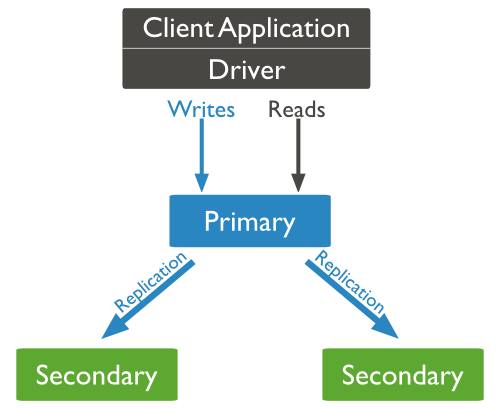
\includegraphics[width=0.95\textwidth]{replication}
  \end{center}
  \caption{MongoDB Replication}
  \label{fig:mongo-replication}
\end{figure}


Replica set features of MonoDB include:

\begin{itemize}
  \item A cluster of N nodes
  \item Any one node can be primary
  \item All write operations go to primary
  \item Automatic failover
  \item Automatic recovery
  \item Consensus election of primary
\end{itemize}

In this tutorial, we will convert standalone MongoDB instance to a
replica set. To convert to replica set, following are the steps:
\begin{enumerate}
  \item Shutdown already running MongoDB server.
  \item Start the MongoDB server by specifying \verb=--replSet= option.
\end{enumerate}


Following is the basic syntax of \verb=--replSet=:

\begin{bashcode}
mongod --port "PORT" --dbpath "YOUR_DB_DATA_PATH" --replSet "REPLICA_SET_INSTANCE_NAME"
\end{bashcode}
It will start a mongod instance with the name rs0, on port 27017.

Now start the command prompt and connect to this mongod instance.

In Mongo client, issue the command \emph{rs.initiate()} to initiate a
new replica set. To check the replica set configuration, issue the
command \emph{rs.conf()}. To check the status of replica set issue the
command rs.status().

To add members to replica set, start mongod instances on multiple
machines. Now start a mongo client and issue a command \emph{rs.add()}
Suppose your mongod instance name is mongod1.net and it is running on
port 27017. To add this instance to replica set, issue the command
\emph{rs.add()} in Mongo client.

\begin{bashcode}
>rs.add("mongod1.net:27017")
>
\end{bashcode}

You can add mongod instance to replica set only when you are connected
to primary node. To check whether you are connected to primary or not,
issue the command \emph{db.isMaster()} in mongo client.

\newpage
\subsection{Sharding}

Sharding is the process of storing data records across multiple machines
and it is MongoDB's approach to meeting the demands of data growth. As
the size of the data increases, a single machine may not be sufficient
to store the data nor provide an acceptable read and write throughput.
Sharding solves the problem with horizontal scaling. With sharding, you
add more machines to support data growth and the demands of read and
write operations.

Benefits of sharding include:
\begin{itemize}
  \item In replication, all writes go to master node
  \item Latency sensitive queries still go to master
  \item Single replica set has limitation of 12 nodes
  \item Memory can't be large enough when active dataset is big
  \item Local disk is not big enough
  \item Vertical scaling is too expensive
\end{itemize}

The following diagram shows the Sharding in MongoDB using sharded cluster.
\begin{figure}[H]
  \begin{center}
    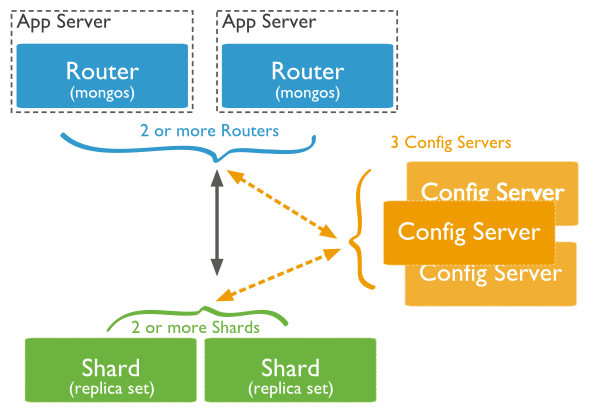
\includegraphics[width=0.95\textwidth]{sharding}
  \end{center}
  \caption{MongoDB Sharding}
  \label{fig:mongo-sharding}
\end{figure}

In the diagram \nameref{fig:mongo-sharding}, there are three main components:
\begin{itemize}
  \item Shards --- Shards are used to store data. They provide high
    availability and data consistency. In production environment, each
    shard is a separate replica set.
  \item Config Servers --- Config servers store the cluster's metadata.
    This data contains a mapping of the cluster's data set to the
    shards. The query router uses this metadata to target operations to
    specific shards. In production environment, sharded clusters have
    exactly 3 config servers.
  \item Query Routers --- Query routers are basically mongo instances,
    interface with client applications and direct operations to the
    appropriate shard. The query router processes and targets the
    operations to shards and then returns results to the clients. A
    sharded cluster can contain more than one query router to divide the
    client request load. A client sends requests to one query router.
    Generally, a sharded cluster have many query routers.
\end{itemize}

\newpage
\subsection{Backup and Restore}

To create backup of database in MongoDB, you may use \emph{mongodump}
command. This command will dump the entire data of your server into the
dump directory. There are many options available by which you can limit
the amount of data or create backup of your remote server.

Assuming that your mongod server is running on the localhost and port
27017, open a command prompt and go to the bin directory of your mongodb
instance and type the command as follows:

\begin{bashcode}
cd /var/lib/mongodb
mongodump -uroot -pexample

2022-05-29T02:40:28.521+0000    writing admin.system.users to dump/admin/system.users.bson
2022-05-29T02:40:28.522+0000    done dumping admin.system.users (1 document)
2022-05-29T02:40:28.522+0000    writing admin.system.version to dump/admin/system.version.bson
2022-05-29T02:40:28.523+0000    done dumping admin.system.version (3 documents)
2022-05-29T02:40:28.523+0000    writing mydb.posts to dump/mydb/posts.bson
2022-05-29T02:40:28.524+0000    done dumping mydb.posts (8 documents)
\end{bashcode}

As indicated by log message, backup files are located under \emph{dump}
directory.

% Following is a list of frequently-used options that can be used with the mongodump command.
% Syntax  Description Example
% mongodump --host HOST_NAME --port PORT_NUMBER   This commmand will backup all databases of specified mongod instance.   mongodump --host tutorialspoint.com --port 27017
% mongodump --dbpath DB_PATH --out BACKUP_DIRECTORY   This command will backup only specified database at specified path. mongodump --dbpath /data/db/ --out /data/backup/
% mongodump --collection COLLECTION --db DB_NAME  This command will backup only specified collection of specified database.   mongodump --collection mycol --db test
% \begin{tabular}{lp{24em}}
%     \bfseries \verb=--host= & Used to select some specific fields from a collection. \\
%     \bfseries \verb=--host= & Used to select some specific fields from a collection. \\
% \end{tabular}

To restore backup data MongoDB's \emph{mongorestore} command is used.
This command restores all of the data from the backup directory. To
restore the backup created previously to the new database \emph{newdb},
you type the command as follows:

\begin{bashcode}
cd /var/lib/mongodb
mongorestore -uroot -pexample --authenticationDatabase admin --nsFrom=mydb.posts --nsTo=newdb.posts

2022-05-29T03:06:21.751+0000    using default 'dump' directory
2022-05-29T03:06:21.751+0000    preparing collections to restore from
2022-05-29T03:06:21.752+0000    reading metadata for newdb.posts from dump/mydb/posts.metadata.json
2022-05-29T03:06:21.773+0000    restoring newdb.posts from dump/mydb/posts.bson
2022-05-29T03:06:21.785+0000    finished restoring newdb.posts (8 documents, 0 failures)
2022-05-29T03:06:21.785+0000    restoring users from dump/admin/system.users.bson
2022-05-29T03:06:21.812+0000    restoring indexes for collection newdb.posts from metadata
2022-05-29T03:06:21.812+0000    index: &idx.IndexDocument{Options:primitive.M{"name":"title_1", "unique":true, "v":2}, Key:primitive.D{primitive.E{Key:"title", Value:1}}, PartialFilterExpression:primitive.D(nil)}
2022-05-29T03:06:21.840+0000    8 document(s) restored successfully. 0 document(s) failed to restore.
\end{bashcode}
The option \verb=--authenticationDatabase admin= is required. Otherwise,
you will run into authentication error.

\subsection{Monitoring}

When you are preparing a MongoDB deployment, you should try to
understand how your application is going to hold up in production. It’s
a good idea to develop a consistent, repeatable approach to managing
your deployment environment so that you can minimize any surprises once
you’re in production.

The best approach incorporates prototyping your set up, conducting load
testing, monitoring key metrics, and using that information to scale
your set up. The key part of the approach is to proactively monitor your
entire system - this will help you understand how your production system
will hold up before deploying, and determine where you will need to add
capacity. Having insight into potential spikes in your memory usage, for
example, could help put out a write-lock fire before it starts.

To monitor your deployment, MongoDB provides \emph{mongostat} and
\emph{mongotop}. The \emph{mongostat} command checks the status of all
running mongod instances and return counters of database operations.
These counters include inserts, queries, updates, deletes, and cursors.
Command also shows when you’re hitting page faults, and showcase your
lock percentage. This means that you're running low on memory, hitting
write capacity or have some performance issue.

To run the command, start your mongod instance. In another command
prompt, go to bin directory of your mongodb installation and type
mongostat as follows:

\pagebreak

\enlargepage
\begin{landscape}
\thispagestyle{empty}
\begin{bashcode}
root@c50373c705ca:/work/.state/mongodb# mongostat -uroot -pexample --authenticationDatabase admin
insert query update delete getmore command dirty used flushes vsize  res qrw arw net_in net_out conn                time
    *0    *0     *0     *0       0     0|0  0.0% 0.0%       0 1.47G 103M 0|0 1|0   111b   47.3k    3 May 29 03:51:47.576
    *0    *0     *0     *0       0     1|0  0.0% 0.0%       0 1.47G 103M 0|0 1|0   112b   47.8k    3 May 29 03:51:48.573
    *0    *0     *0     *0       0     0|0  0.0% 0.0%       1 1.47G 103M 0|0 1|0   111b   47.5k    3 May 29 03:51:49.575
    *0    *0     *0     *0       0     1|0  0.0% 0.0%       0 1.47G 103M 0|0 1|0   112b   47.7k    3 May 29 03:51:50.574
    *0    *0     *0     *0       0     1|0  0.0% 0.0%       0 1.47G 103M 0|0 1|0   112b   47.6k    3 May 29 03:51:51.574
    *0    *0     *0     *0       0     1|0  0.0% 0.0%       0 1.47G 103M 0|0 1|0   112b   47.7k    3 May 29 03:51:52.573
    *0    *0     *0     *0       0     0|0  0.0% 0.0%       0 1.47G 103M 0|0 1|0   111b   47.6k    3 May 29 03:51:53.574
    *0    *0     *0     *0       0     1|0  0.0% 0.0%       0 1.47G 103M 0|0 1|0   112b   47.7k    3 May 29 03:51:54.573
    *0    *0     *0     *0       0     1|0  0.0% 0.0%       0 1.47G 103M 0|0 1|0   112b   47.7k    3 May 29 03:51:55.573
    *0    *0     *0     *0       0     2|0  0.0% 0.0%       0 1.47G 103M 0|0 1|0   307b   48.2k    3 May 29 03:51:56.573
insert query update delete getmore command dirty used flushes vsize  res qrw arw net_in net_out conn                time
    *0    *0     *0     *0       0     0|0  0.0% 0.0%       0 1.47G 103M 0|0 1|0   111b   47.6k    3 May 29 03:51:57.574
    *0    *0     *0     *0       0     1|0  0.0% 0.0%       0 1.47G 103M 0|0 1|0   112b   47.7k    3 May 29 03:51:58.573
    *0    *0     *0     *0       0     0|0  0.0% 0.0%       0 1.47G 103M 0|0 1|0   111b   47.6k    3 May 29 03:51:59.574
    *0    *0     *0     *0       0     1|0  0.0% 0.0%       0 1.47G 103M 0|0 1|0   112b   47.7k    3 May 29 03:52:00.573
    *0    *0     *0     *0       0     0|0  0.0% 0.0%       0 1.47G 103M 0|0 1|0   111b   47.6k    3 May 29 03:52:01.574
    *0    *0     *0     *0       0     1|0  0.0% 0.0%       0 1.47G 103M 0|0 1|0   112b   47.7k    3 May 29 03:52:02.573
\end{bashcode}
\end{landscape}
\restorepage

Please be advised that command line switches are version specific. 
For mongodb 4.x, the option \emph{--authenticationDatabase admin} is
required to work with mongodb with authencation enabled.


The \emph{mongotop} command tracks and reports the read and write
activity of MongoDB instance on a collection basis. By default,
\emph{mongotop} returns information in each second, which you can change
it accordingly. To change mongotop command to return information less
frequently, specify a specific number after the mongotop command. You
should check that this read and write activity matches your application
intention, and you’re not firing too many writes to the database at a
time, reading too frequently from a disk, or are exceeding your working
set size.

To run the command, start your mongod instance. In another command
prompt, go to bin directory of your mongodb installation and type
mongotop.


\begin{bashcode}
root@c50373c705ca:/work/.state/mongodb# mongotop -uroot -pexample --authenticationDatabase admin
2022-05-29T03:53:27.505+0000    connected to: mongodb://localhost/

                    ns    total    read    write    2022-05-29T03:53:28Z
    admin.system.roles      0ms     0ms      0ms
    admin.system.users      0ms     0ms      0ms
  admin.system.version      0ms     0ms      0ms
config.system.sessions      0ms     0ms      0ms
   config.transactions      0ms     0ms      0ms
  local.system.replset      0ms     0ms      0ms
            mydb.posts      0ms     0ms      0ms
           newdb.posts      0ms     0ms      0ms

                    ns    total    read    write    2022-05-29T03:53:29Z
    admin.system.roles      0ms     0ms      0ms
    admin.system.users      0ms     0ms      0ms
  admin.system.version      0ms     0ms      0ms
config.system.sessions      0ms     0ms      0ms
   config.transactions      0ms     0ms      0ms
  local.system.replset      0ms     0ms      0ms
            mydb.posts      0ms     0ms      0ms
           newdb.posts      0ms     0ms      0ms
\end{bashcode}

\newpage
\section{Programming}
\subsection{Java}
\subsection{PHP}
\subsection{golang}

\newpage
\section{Reference}
\subsection{Useful Resources}

\end{document}
% vim: set ai nu nobk expandtab ts=4 sw=2 tw=72 syntax=tex :
